\documentclass[11pt]{article}
\usepackage[margin=0.85in]{geometry}
\usepackage{amsmath}
\usepackage{amssymb}
\usepackage{booktabs}
\usepackage{caption}
\usepackage{graphicx}
\usepackage{xcolor}
\usepackage{titlesec}
\titlespacing*{\section}{0pt}{1.0ex plus .2ex minus .2ex}{0.6ex plus .2ex}
\setlength{\parskip}{0pt}
\usepackage[colorlinks=true,linkcolor=blue,urlcolor=blue]{hyperref}

\title{\vspace{-1.5em}Gated Depth-Readers Lose to Deeper Trunks:\\
       a per-FLOP study at $d{=}10$\vspace{-0.5em}}
\author{2d-Transformers}
\date{June 25, 2026}

\newcommand{\bpb}{\textsc{bpb}}

\begin{document}
\maketitle
\vspace{-1em}

\section{Motivation}

A depth-$L$ transformer builds a \emph{residual stream}: starting from the token embedding $x_0$, each
layer adds its update, producing a ladder of hidden states
\[
\Lambda \;=\; [\,x_0,\; h_1,\; h_2,\; \dots,\; h_L\,] \qquad (L{+}1 \text{ ``rungs''}).
\]
A standard model reads out only the \textbf{top rung} $h_L$ through the language-model head. But the
intermediate rungs hold features at different levels of abstraction, and $h_L$ is a single-vector
bottleneck. This raises a natural question:

\begin{quote}
\emph{Can a model produce a better readout by reading its \textbf{entire depth} $\Lambda$, rather than
just the last layer?}
\end{quote}

Six earlier experiments tested a \emph{depth-reader} that \textbf{replaces} $h_L$ (it ``owns'' the
output). It never beat the plain top-state baseline. Replacing a good representation may be too
aggressive --- so here we test the gentlest possible version: the reader as a small, \textbf{gated
additive correction} to $h_L$, which at initialization changes nothing and must \emph{earn} its
influence.

\section{Architecture: the gated depth-reader}

On top of the usual backbone $H$ (depth $L$, width $e$) we add a small reader $V$:

\begin{itemize}\itemsep2pt
  \item \textbf{Reader $V$.} A small transformer of $V$ blocks at full width $e$ (same block shape as
  the backbone). It attends over the \emph{depth} axis --- the $L{+}1$ rungs of $\Lambda$ are treated
  as a sequence --- and returns a correction vector $r = V(\Lambda)$.
  \item \textbf{Gated readout.} Instead of $x = h_L$, the model uses
  \[
  \boxed{\;\text{readout} \;=\; \underbrace{h_L}_{\text{baseline top state}} \;+\; g\cdot V(\Lambda)\;}
  \qquad g\in\mathbb{R},\quad g_0 = 10^{-3}.
  \]
  \item \textbf{The gate $g$} is a single scalar, initialized $\approx 0$, with its own optimizer
  group, logged at every evaluation.
\end{itemize}

The design makes the comparison honest. At $g{=}0$ the model is \emph{exactly} the baseline, so the
reader can never start out worse. The tiny $g_0$ still gives $V$ a gradient from step $0$, so it
learns immediately. If reading the ladder helps, $g$ grows and we see it; if it does not, $g$ stays
near zero. ``Did the reader turn on?'' becomes a \emph{measured} quantity, not an assumption.

\section{Experiment: the V-slope at $d{=}10$}

We fix the backbone at $d{=}10$ ($e{=}640$) and sweep the reader depth
$V \in \{2,4,8,10\}$, all gated. Every model is trained compute-optimally (tokens $= 12\times$ params).
A reader is a \emph{bigger} model ($H{+}V$ parameters), so it is fairly given proportionally more
tokens.

The decisive question is \textbf{per-FLOP}: for the same total compute, you could instead train a
\emph{deeper plain transformer}. So we also train plain baselines $d{=}12,14,16$ (and reuse $d{=}10$),
giving a loss-versus-compute \textbf{frontier}. The verdict for each reader is simply: does it land
\emph{below} that frontier (a per-compute win) or \emph{above} it (a loss)? Quality is validation
bits-per-byte (\bpb, lower is better).

\section{Results}

\begin{table}[h]
\centering
\begin{minipage}{0.46\textwidth}\centering
\caption*{\textbf{Plain baseline frontier}}
\begin{tabular}{lrr}
\toprule
model & total FLOPs & \bpb \\
\midrule
$d{=}10$ & $0.49\times10^{18}$ & 0.8769 \\
$d{=}12$ & $1.17\times10^{18}$ & 0.8307 \\
$d{=}14$ & $2.55\times10^{18}$ & 0.7967 \\
$d{=}16$ & $5.11\times10^{18}$ & \textbf{0.7737} \\
\bottomrule
\end{tabular}
\end{minipage}\hfill
\begin{minipage}{0.52\textwidth}\centering
\caption*{\textbf{Gated readers} (vs.\ frontier at equal FLOPs)}
\begin{tabular}{lrrr}
\toprule
reader & \bpb & frontier & gap \;/\; gate \\
\midrule
$V{=}2$  & 0.8665 & 0.834 & \textcolor{red}{$+0.033$} \;/\; 0.40 \\
$V{=}4$  & 0.8570 & 0.810 & \textcolor{red}{$+0.047$} \;/\; 0.35 \\
$V{=}8$  & 0.8431 & 0.779 & \textcolor{red}{$+0.064$} \;/\; 0.39 \\
$V{=}10$ & 0.8376 & 0.768 & \textcolor{red}{$+0.070$} \;/\; 0.40 \\
\bottomrule
\end{tabular}
\end{minipage}
\end{table}

\begin{figure}[h]
\centering
\vspace{-0.5em}
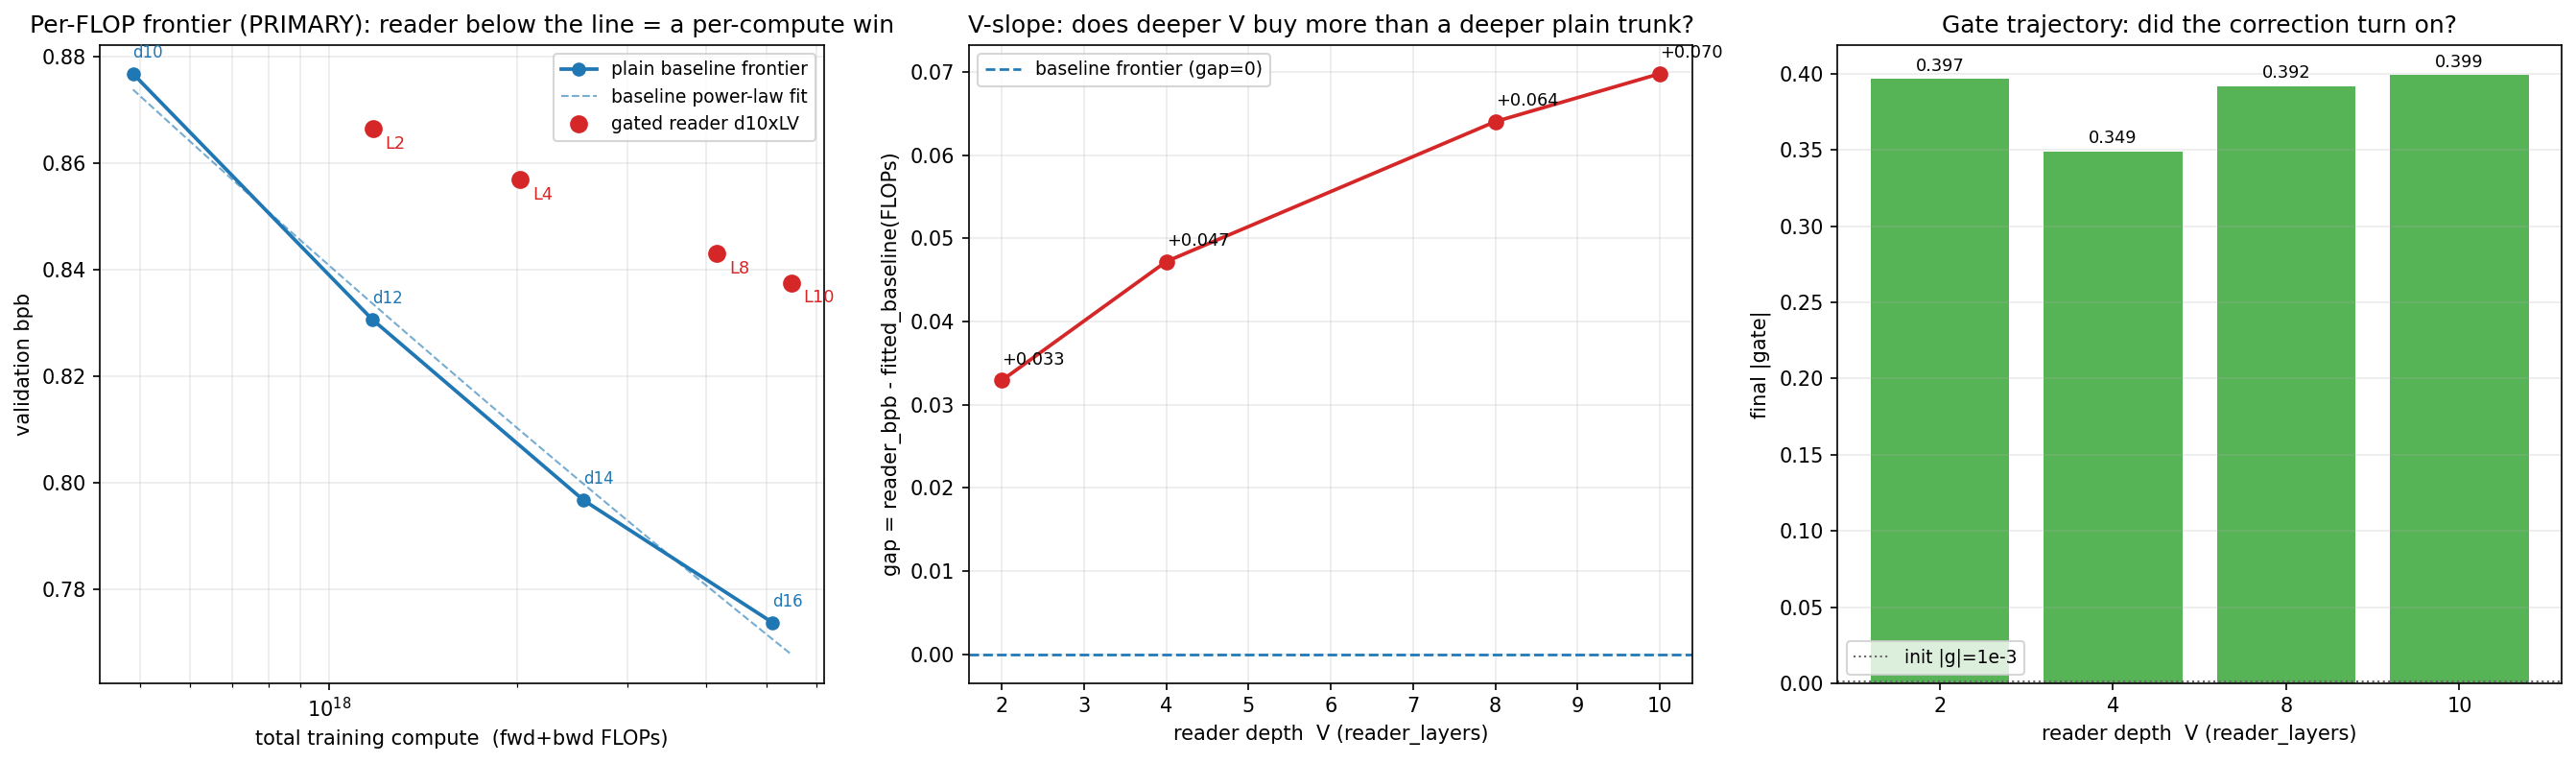
\includegraphics[width=0.82\textwidth]{figs/hv_sweep.png}
\vspace{-0.7em}
\caption{\textbf{Left:} the four plain baselines (blue) trace a loss-vs-compute frontier; all four
gated readers (red) sit \emph{above} it --- a per-compute loss at every depth. \textbf{Middle:} the
gap to the frontier \emph{grows} with reader depth. \textbf{Right:} the gate is firmly on
($|g|\approx 0.35$--$0.40$, from a $10^{-3}$ init) in every run --- the reader genuinely turned on.}
\end{figure}

Three things stand out:
\begin{enumerate}\setlength{\itemsep}{1pt}\setlength{\parsep}{0pt}\setlength{\topsep}{2pt}
  \item \textbf{Every reader loses per-FLOP}, and the gap \emph{widens} with $V$ ($+0.033 \to +0.070$
  \bpb). At $\sim\!5\times10^{18}$ FLOPs, a plain $d{=}16$ scores $0.774$ while the deepest reader
  ($V{=}10$) reaches only $0.838$ --- the baseline wins by $0.064$. Plain depth scales $\sim\!3\times$
  better per FLOP.
  \item \textbf{It is not a dead component.} The gate turned on hard in every run, so the reader
  \emph{did} learn and contribute. This is a real negative result, not an artifact of $V$ doing
  nothing.
  \item \textbf{The ``equal-data'' win is a mirage.} The readers do beat the $d{=}10$ anchor
  ($0.877$) token-for-token --- but only because they are bigger models fed more tokens. Matched on
  \emph{compute}, they lose.
\end{enumerate}

\section{Conclusion}

Even in its most favorable form --- additive, gated, and free to learn to turn itself on --- the
depth-reader is a \textbf{worse use of compute than simply making the trunk deeper}, and
\emph{increasingly so} with reader depth. The takeaway is blunt: spend the FLOPs on depth, not on
re-reading the ladder.

\end{document}
